%%%%%%%%%%%%%%%%%%%%%%%%%%%%%%%%%%%%%%%%%
% Developer CV
% LaTeX Template
% Version 1.0 (28/1/19)
%
% This template originates from:
% http://www.LaTeXTemplates.com
%
% Authors:
% Jan Vorisek (jan@vorisek.me)
% Based on a template by Jan Küster (info@jankuester.com)
% Modified for LaTeX Templates by Vel (vel@LaTeXTemplates.com)
%
% License:
% The MIT License (see included LICENSE file)
%
%%%%%%%%%%%%%%%%%%%%%%%%%%%%%%%%%%%%%%%%%

%----------------------------------------------------------------------------------------
%	PACKAGES AND OTHER DOCUMENT CONFIGURATIONS
%----------------------------------------------------------------------------------------

\documentclass[9pt]{developercv} % Default font size, values from 8-12pt are recommended

%----------------------------------------------------------------------------------------

\begin{document}
	
	%----------------------------------------------------------------------------------------
	%	TITLE AND CONTACT INFORMATION
	%----------------------------------------------------------------------------------------
	
	\begin{minipage}[t]{0.45\textwidth} % 45% of the page width for name
		\vspace{-\baselineskip} % Required for vertically aligning minipages
		

			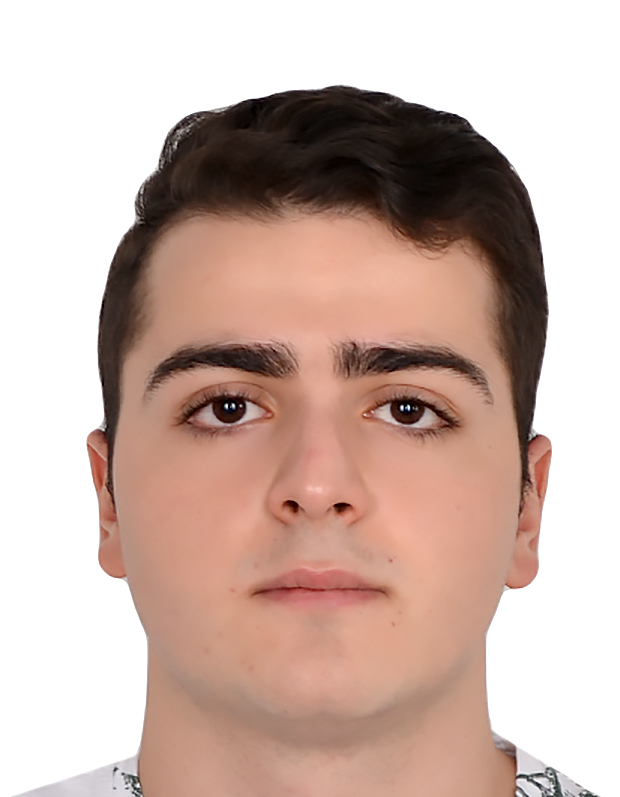
\includegraphics[scale=0.65]{photo.jpg}

		\huge{David Kagramanyan} % Last name
		
		\vspace{6pt}
		
		{\huge Junior Data Scientist\\}
		\normalsize{internship, part-time}
		
		
	
	\end{minipage}
	\begin{minipage}[t]{0.4\textwidth} % 27.5% of the page width for the first row of icons
		\vspace{-\baselineskip} % Required for vertically aligning minipages
		
		% The first parameter is the FontAwesome icon name, the second is the box size and the third is the text
		% Other icons can be found by referring to fontawesome.pdf (supplied with the template) and using the word after \fa in the command for the icon you want
		
		\icon{At}{11}{\href{mailto:dgkagramanyan@miem.hse.ru}{dgkagramanyan@miem.hse.ru}}\\	
		\icon{Github}{11}{\href{https://github.com/ArmageddonReloadedDK}{github.com/ArmageddonReloadedDK}}\\
		
	\end{minipage}
	\begin{minipage}[t]{0.5\textwidth} % 27.5% of the page width for the second row of icons
		\vspace{-\baselineskip} % Required for vertically aligning minipages
		% The first parameter is the FontAwesome icon name, the second is the box size and the third is the text
		% Other icons can be found by referring to fontawesome.pdf (supplied with the template) and using the word after \fa in the command for the icon you want
		
		\icon{Phone}{12}{+79661167186}\\
		\icon{MapMarker}{12}{Moscow}\\
		
		
	\end{minipage}
	
	\vspace{0.5cm}
	
	%----------------------------------------------------------------------------------------
	%	INTRODUCTION, SKILLS AND TECHNOLOGIES
	%----------------------------------------------------------------------------------------
	
	

	\cvsect{Education}

\begin{entrylist}
	\entry
	{2018 -- 2022}
	{Bachelor - HSE Tikhonov Moscow Institute of Electronics and Mathematics}
	{ }
	{Information Science and Computation Technology (School of Computer Engineering)}
	\entry
	{2021}
	{Coursera - Deeplearning.ai}
	{ }
	{\href{https://coursera.org/share/1d45e9d0ba15647e611293d3955245dc}{Specialization TensorFlow: Advanced Techniques}}
	
	\entry
	{2020}
	{Coursera - MIPT}
	{ }
	{\href{https://coursera.org/share/bafe4bd915f06b8a8dce179ffabdbd22}{Mathematics and Python for data science}}
	
\end{entrylist}
	
	
	%----------------------------------------------------------------------------------------
	%	EXPERIENCE
	%----------------------------------------------------------------------------------------
	
	\cvsect{Experience}
	
	\begin{entrylist}
		\entry
		{02.2020 - 12.2020}
		{Mathematical analysis study assistant - HSE Tikhonov Moscow Institute of Electronics and Mathematics}
		{ }
		{Grading test papers, oral tests }
	\end{entrylist}
	
	%----------------------------------------------------------------------------------------
	%	EDUCATION
	%----------------------------------------------------------------------------------------
	
	\cvsect{Skills}
	
	\begin{entrylist}
		\entry
		{ }
		{Mathematical base}
		{ }
		{Mathematical analysis, statistics, linear algebra, probability theory    }
		\entry
		{ }
		{Languages }
		{ }
		{Python 1 year+, C++ (basics), SQL }
		\entry
		{ }
		{Frameworks and libraries}
		{ }
		{Tensorflow (Keras) 1 year+, numpy, pandas, matplotlib }
		\entry
		{ }
		{Fields of interest}
		{ }
		{Computer vision (segmentation, classification, detection, image generation) and  nlp using neural networks  }
		\entry
		{ }
		{Studied aproaches and models}
		{ }
		{Word2vec, cbow, vgg, resnet, gan, siameses, Bert    }
		\entry
		{ }
		{Other}
		{ }
		{Git, Latex, Sphinx, Unix (base) }
	\end{entrylist}

	\cvsect{Projects}
	
	\begin{entrylist}
		\entry
		{CV }
		{Person face classification on VGG16}
		{ }
		{\href{https://github.com/ArmageddonReloadedDK/face_net}{Repository}. Role - main developer. Result - classifying model with categorical accuracy 0.7 on 13 classes }
		\entry
		{CV}
		{Pokemon image generation on GAN}
		{}
		{\href{https://github.com/ArmageddonReloadedDK/piko_gan}{Repository}.  Role - main developer. Result - creating an abstact
		 pokemon image model }
		\entry
		{NLP}
		{Horoscope generaion}
		{ }
		{\href{https://github.com/ArmageddonReloadedDK/astro}{Repository} Role - main developer. Result - model that generates horoscopes  }
	
	\end{entrylist}
	
	%----------------------------------------------------------------------------------------
	%	ADDITIONAL INFORMATION
	%----------------------------------------------------------------------------------------
	
	\begin{minipage}[t]{0.3\textwidth}
		\vspace{-\baselineskip} % Required for vertically aligning minipages
		
		\cvsect{Languages}
		
		\textbf{English} - Upper-ntermediate, reading scientific abstracts\\
		\textbf{Russian} - Native\\
		\textbf{Armenian} - Native\\
	\end{minipage}
	\hfill
	\begin{minipage}[t]{0.3\textwidth}
		\vspace{-\baselineskip} % Required for vertically aligning minipages
		
		\cvsect{Hobbies}
		
		Electronic, working with hands, sport
	\end{minipage}
	\hfill
	
	
	%----------------------------------------------------------------------------------------
	
\end{document}
